\chapter{Stand van zaken}
\label{ch:stand-van-zaken}
\section{Spraakgestuurde technologie}
Er zijn enkele begrippen die met het thema te maken hebben, maar die niet hetzelfde omvatten. Taal- en spraaktechnologie is een verzamelnaam voor allerlei technieken waarmee de computer communiceert met zijn gebruiker door menselijke taal.\autocite{Taalunie2017} Het is de poging van de computer om de menselijke taal na te bootsen.

Spraaktechnologie wordt vaak geassocieerd met spraakherkenning. Volgens \autocite{Rouse2016} is spraakherkenning de kunst van de computer om gesproken taal te identificeren en om te zetten naar voor de computer leesbare machinetaal. Dit is echter maar één techniek die gebruikt wordt binnen de spraaktechnologie. Een tweede techniek, die net het omgekeerde is van spraakherkenning, is spraaksynthese. Volgens dezelfde bron is spraaksynthese menselijke spraak dat is ontwikkeld door een computer. Het wordt gebruikt om geschreven tekst om te zetten naar gesproken taal, geproduceerd door de computer.

Spraaktechnologie omvat naast deze twee begrippen nog meer. Denk maar aan spelling- en grammaticacontrole, spraak- en tekstanalyse, automatische vertalingen, enzovoort.

Spraakherkenning en spraaksynthese zijn nodig in het ontwikkelen van een Voice User Interface (VUI), of stemgestuurde gebruikersomgeving, waar de gebruiker de computer als het ware bedient met zijn stem in plaats van bijvoorbeeld een toetsenbord of aanrakingen. De computer moet gesproken taal van de gebruiker begrijpen (spraakherkenning) en moet een gepast antwoord teruggeven (spraaksynthese). Spraakassistenten zoals Alexa, Siri of Google Assistant zijn voorbeelden van VUI's.

\section{Spraakassistenten}
Een spraakassistent, ook wel een virtuele, persoonlijke of slimme assistent genoemd, voert taken uit via verbale instructies van een gebruiker. Het is vooral aanwezig in smartphones, maar het wordt ook geïntegreerd in smart speakers, auto's of wearables. Dit onderzoek vergelijkt twee van de meest prestigieuze assistenten, Google’s Assistant en Amazon’s Alexa. Daarnaast zijn ook Apple's Siri, Microsoft's Cortana en Samsung's Bixby bekende voorbeelden.

\subsection{De geschiedenis van spraakassistenten}
De slimme spraakassistenten zijn vandaag gekend bij het grote publiek. Ze zijn ingebouwd in onze smartphones en slimme luidsprekers. Steeds paraat om ons de vertragingen te melden op de weg, het weer te voorspellen voor morgen of onze favoriete muziek te spelen. Het is iets van deze tijd, maar toch hebben ze al een lang pad van tientallen jaren bewandeld. Dit is hoe het allemaal begon en hoe we zijn geëvolueerd naar de bekende assistenten van vandaag.

\subsubsection{Jaren 50 - 60}
De eerste systemen die ietwat leken op een spraakassistent waren gefocust op het louter herkennen van de menselijke spraak. In \autocite{Vox-Creative2019} wordt geschreven hoe in  de Bell Laboratories in 1952 het ``Audrey'' systeem werd ontwikkeld. Audrey begreep de getallen 0 tot 9 op voorwaarde dat de sprekers tussen elk getal een pauze lieten. In theorie kon het gebruikt worden om met de stem een telefoonnummer in te geven. Onder andere de kost en omvang van de machine was groot. Het intoetsen van de telefoonknoppen bleef efficiënter, dus het effectieve gebruik van Audrey bleef uit.

\autocite{IBM2011} onthulde in 1962 de ``Shoebox'', een machine die met spraakcommando's eenvoudige berekeningen kon uitvoeren. De uitvinder William C. Dersch demonstreerde voor televisie hoe het apparaat, zo groot als een schoendoos, naast de getallen 0 tot 9 ook zes woorden zoals plus en totaal kon herkennen.

\begin{figure}[h]
    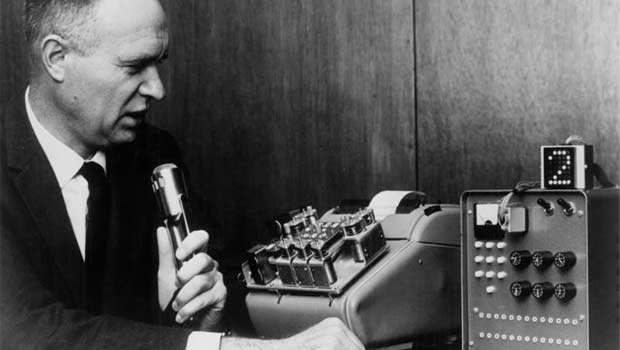
\includegraphics[width=0.7\linewidth]{img/Shoebox}
    \caption{William C. Dersch’s Shoebox deed eenvoudige berekeningen met spraakcommando's \autocite{IBM2011}}
    \label{fig:smartassist}
\end{figure}

\subsubsection{Jaren 70 - 80}
Spraakherkenning in de jaren 70 werd vooral gekenmerkt door het departement voor defensie in de Verenigde Staten. Uit interesse voor spraakherkenning financierden ze een vijfjarig project over het thema. Volgens \autocite{Pinola2011} en \autocite{Kincaid2018} heeft dit geleid tot de ontwikkeling van Harpy in 1976. Harpy begreep 1011 woorden en kreeg vooral betekenis door haar efficiëntere zoekmethode, de ``Beam-search'', om logische zinnen te gaan herkennen.

In \autocite{Pinola2011} staat dat in de jaren 80 er een grote doorbraak kwam door de ontwikkeling van het hidden Markov model. Dit model gebruikt statistieken om een woord te herkennen in een onbekend geluid. Dit werd gedaan door het berekenen van de waarschijnlijkheid dat het onbekend geluid staat voor een bepaald woord. De woordenschat van de spraakherkenningssoftware bleef groeien tot een paar duizend woorden en had dankzij onder andere het hidden Markov model het potentieel om ongelimiteerd woorden te gaan herkennen.
Onder andere dankzij deze ontwikkelingen bleven ook de commerciële toepassingen niet uit. In 1987 kwam de Worlds of Wonder's doll Julie uit. Kinderen konden de pop trainen om te reageren op hun uitspraken. Dit staat zo beschreven in \autocite{Pinola2011}, waar je ook een reclamespot voor de pop kan bekijken. De technologie groeide snel, maar had wel een grote zwakte. De zin moest gedicteerd worden. Na elk woord werd dus een korte pauze verwacht.

\subsubsection{Jaren 90}
Volgens \autocite{Kincaid2018} kwam in de 90's automatische spraakherkenning in een eerste vorm zoals we het vandaag kennen. De doorbraak in die tijd heette Dragon. De eerste versie werd gelanceerd in 1990 onder de naam Dragon Dictate en had een woordenschat van 80 000 woorden. Daarnaast kon het iets nieuws, iets wat in de huidige spraakassistenten nog steeds gebruikt wordt, natural language processing. Zinnen moesten niet meer gedicteerd worden, maar Dragon kon oorspronkelijk 30 tot 40 woorden per minuut herkennen.

Volgens een artikel uit 1998 \autocite{Puri1998} is Dragon verantwoordelijk voor een doorbraak in spraakherkenningssoftware. De opvolger van de Dragon Dictate, Dragon NaturallySpeaking laat gebruikers spreken in een microfoon, aangesloten op de computer, en laat de woorden direct verschijnen op het computerscherm. Indien het een fout maakte, kon je het zelf corrigeren en kon de software leren uit zijn fouten. Het was ook de eerste spraakherkenningssoftware die toeliet om op een normale manier te praten.

\subsubsection{Van 2010 tot nu}
In \autocite{IBM2011} is te lezen hoe een mijlpaal werd bereikt door de Watson machine die won in Jeopardy. Watson was zo goed in taalverwerking dat hij 2 kampioenen in Jeopardy heeft verslaan live op televisie. Jeopardy is een Amerikaans spelprogramma waar de kandidaten het antwoord kregen en ze zelf de bijpassende vraag moesten geven. Watson was niet alleen goed in het samenstellen van correcte vragen, maar kon die ook telkens hardop uitspreken.

\begin{figure}[h]
    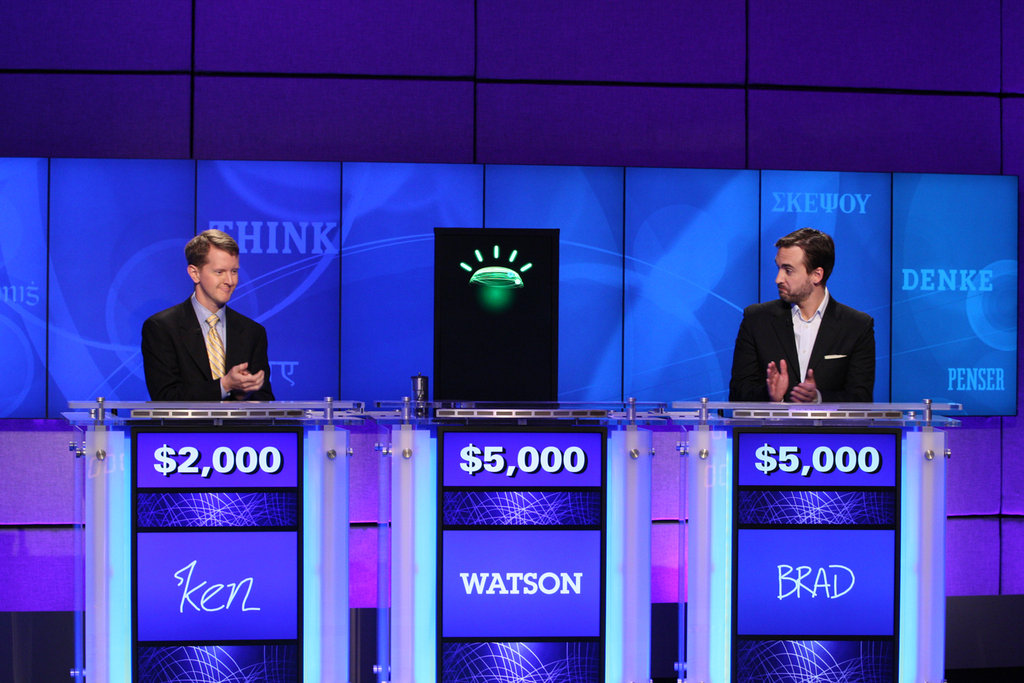
\includegraphics[width=0.7\linewidth]{img/WatsonJeopardy}
    \caption{Watson versloeg twee kampioenen in Jeopardy live op televisie \autocite{Markoff2011}}
    \label{fig:smartassist}
\end{figure}

Kort na deze gebeurtenis in 2011 werd Siri geïntegreerd in de Iphone 4S en werd zo de eerste spraakassistent voor het grote publiek uitgebracht. Google gaf hierop een antwoord in 2012 door Google Now uit te brengen, de voorloper van de Google Assistant van vandaag. Tijdens de Microsoft BUILD conferentie in 2013 werd Cortana geïntroduceerd als de spraakassistent van Microsoft. In 2015 kwam de eerste slimme luidspreker op de markt. De Echo van Amazon, voorzien met hun slimme spraakassistent, Alexa.

\subsection{Hoe werkt een spraakassistent}

\subsection{De spraakassistenten van nu}
Volgens Google is de Google Assistant jouw eigen persoonlijke Google, die altijd bereid is om je te helpen wanneer je maar wilt. De Google Assistant bestond eerst onder de naam Google Now en was aanwezig in smartphones met een Android besturingssysteem. De Google Assistant van vandaag is te vinden in veel meer omgevingen. Smartphones, auto's, laptops, tablets, tv's, smartwatches en in hun eigen smart speaker, de Google Home. Deze speaker heeft ook een variant gekregen met een scherm, de Smart Display.
[bron 1e paper] evalueerde verschillende functionaliteiten van spraakassistenten Google Assistant, Alexa en Siri, op correctheid en natuurlijkheid bij 8 ondervraagden. In de administratieve categorie, zoals agendabeheer, to-do-lijsten en alarmen kwam de Google Assistent als minst correct en minst natuurlijke assistant uit de bus, maar prijkt in de miscallenous category (nieuws, weer, verkeer, woordbetekenissen, rekenen,, enz.) dan weer ver bovenaan op beide vlakken. Algemeen werd de Google Assistant als de meest natuurlijke ervaren, onder andere door de toon van de stem die surprise, suspense en joy uitte.
Voor [bron 2e paper] stelden 100 personen allerlei vragen aan voice assistants Google Assistant, Alexa, Siri en Cortana. Ze gaven telkens een score op spraakherkenning en contextueel inzicht. Google Assistant kwam als grote winnaar uit het onderzoek door 59,80 \% van de vragen te beantwoorden. Een verschil van 15,82 \% met Siri, die de op één na nauwkeurigste bleek in dit onderzoek. Google Assistant was vooral leider in categoriëen als reizen, emailing, navigatie, vertalingen en begreep volgens het onderzoek goed de verschillende variaties in de stemmen van de onderzochte personen.

Amazon, één van 's werelds grootste bedrijven in het online verkopen van goederen, is ook met een spraakassistent op de markt gekomen. Het grote verschil met Google is dat de assistent voor het eerst werd gebruikt in de Echo, Amazon's smart speaker. Volgens [bron 1e paper] is de Echo Dot de favoriete smart speaker als het aankomt op het aankopen van artikelen. Dit is geen verrassing aangezien hij oorspronkelijk ontworpen is om te winkelen en zelfs de enige spraakassistent is waarmee je online kan shoppen. In [bron 2e paper] bleek Alexa de minst nauwkeurige assistant te zijn met 7,91 \% nauwkeurigheid.

Slimme spraakassistenten worden alleen maar slimmer. [bron4] heeft onderzocht hoe hoog het intelligentieniveau is van 4 slimme assistenten, namelijk Google Assistant, Microsoft Cortana, Amazon Alexa en Apple Siri in 2017 en 2018. De geanalyseerde gegevens zijn de antwoorden van de assistenten op 5000 algemene vragen. De beste prestatie werd verricht door Google Assistant die op 77,2 procent van de vragen een antwoord kon bieden, waarvan 95 procent correct. Bij alle assistenten zie je een verhoging van de intelligentie in vergelijking met het vorige jaar.

\begin{figure}[h]
    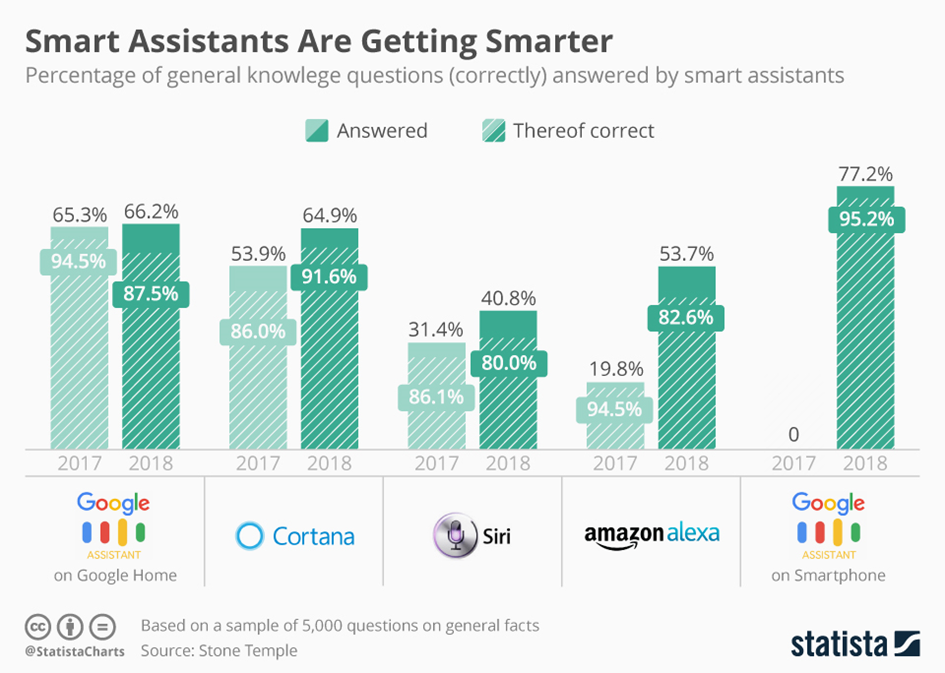
\includegraphics[width=0.7\linewidth]{img/SmartAssistantsAreGettingSmarter}
    \caption{Hoe hoog ligt het intelligentieniveau bij slimme spraakassistenten}
    \label{fig:smartassistantsaregettingsmarter}
\end{figure}


\section{Eerste hulp bij ongevallen}
De AED of automatische externe defibrillator is een toestel dat een elektrische schok geeft om het hartritme te herstellen bij een hartaanval. Om verwarring te vermijden, bij een hartstilstand staat het hart niet echt stil, maar stopt het met functioneren door het gevolg van hartritmestoornissen. Defibrilleren doet het hart echter wel stilstaan, zodanig dat de normale hartmechanismen de controle opnieuw kunnen overnemen. [bron3] Volgens [bron1] heeft het belang van vroegtijdig defibrilleren voor het verhogen van de overlevingskans geleid tot het concept van de ‘eerste hulp’-defibrillatie en het AED toestel. Tegenwoordig zijn er in België AED’s voorzien op verschillende openbare plaatsen zoals sporthallen, scholen of grote bedrijven om er voor zorgen dat defibrillatie vroegtijdig kan uitgevoerd worden door niet-medisch personeel, in afwachting van de komst van getraind medisch personeel.

Onderzoeken die het nut aantonen van eerste hulp enzo.

\section{Bestaande eerste hulpapplicaties}
\subsection{De Vlaamse EHBO-app van het Rode Kruis}
Op 2 april ’19 kwam het Rode Kruis met het nieuws dat ze een app hebben ontwikkeld die kan helpen bij het geven van eerste hulp bij ongevallen. 80 procent van de Vlamingen weet niet wat hij moet doen als een nabije persoon begint te stikken, een hartstilstand krijgt of hevig begint te bloeden. Uit angst om iets fouts te doen, gebeurt er dan ook vaak niks. Met de app willen ze zoveel mogelijk mensen in staat stellen om hulp te verlenen. [bron2]

Het Rode Kruis benadrukt dat de applicatie de opleiding niet kan vervangen, maar dat het hulp kan bieden bij het geven van eerste hulp.

In de applicatie zijn er drie grote onderdelen, eerste hulp verlenen, eerste hulp leren en een AED-toestel vinden in de buurt. Er zijn ook nog enkele opties die je naar de website van het Rode Kruis brengen om informatie te verkrijgen over het geven van bloed of plasma, het doen van een gift, het volgen van een opleiding of het aanmelden als vrijwilliger.

Als je eerste hulp wilt verlenen kun je uit het overzicht een onderwerp over eerste hulp kiezen, waarna je informatie krijgt over wat je moet vaststellen en wat je nodig hebt. Daarnaast geeft de app ook een stappenplan van instructies wat je moet doen. De levensbedreigende situaties staan helemaal bovenaan en zijn voorzien van extra ingesproken instructies.

Als je eerste hulp wilt leren kun je eerst een onderwerp kiezen. Voorbeelden zijn een beroerte of alcoholvergiftiging. Daarna krijg je over het onderwerp vragen \& antwoorden, informatieteksten en video's. Per leerdeel krijg je een quiz die je moet oplossen om bepaalde badges te verdienen.

Wanneer iemand in uw omgeving een hartstilstand krijgt dan kun je met de applicatie een kaart openen waar AED-toestellen staan op gesitueerd. Je kunt er ook een nieuwe AED melden of meer informatie lezen.


\subsection{Andere EHBO-applicaties}
Nederland heeft al langer een mobiele EHBO-applicatie. Deze verschilt niet zo veel met de Belgische versie. Ze heeft wel een zoekfunctie om sneller de instructies voor uw ongeval te vinden. Je kan er ook EHBO-kits en cursussen bestellen in de webshop.
